% Created 2013-01-25 Fri 08:22
\documentclass[table]{beamer}
\usepackage[utf8]{inputenc}
\usepackage[T1]{fontenc}
\usepackage{fixltx2e}
\usepackage{graphicx}
\usepackage{longtable}
\usepackage{float}
\usepackage{wrapfig}
\usepackage{soul}
\usepackage{textcomp}
\usepackage{marvosym}
\usepackage{wasysym}
\usepackage{latexsym}
\usepackage{amssymb}
\usepackage{hyperref}
\tolerance=1000
\usepackage{tikz}
\usepackage{minted}
\usepackage{fancyvrb}
\usemintedstyle{perldoc}
\definecolor{lightgray}{gray}{0.96}
\setlength{\tabcolsep}{1ex}
\institute{Harvard MIT Data Center}
\usetheme{Warsaw}
\useoutertheme{infolines}
\setbeamercolor{block body}{bg=lightgray}
\titlegraphic{
\includegraphics[width=.75\textwidth]{images/IQSSNewLogo.pdf}}
\AtBeginSection[]{\begin{frame}<beamer>\frametitle{Topic}\tableofcontents[currentsection]\end{frame}}
\providecommand{\alert}[1]{\textbf{#1}}

\title{Graphing in Stata}
\author{Ista Zahn}
\date{January 25 2013}
\hypersetup{
  pdfkeywords={},
  pdfsubject={},
  pdfcreator={Emacs Org-mode version 7.9.3d}}

\begin{document}

\maketitle

\begin{frame}
\frametitle{Outline}
\setcounter{tocdepth}{3}
\tableofcontents
\end{frame}







\section{Introduction}
\label{sec-1}

\rowcolors{1}{blue!15}{blue!3}
\definecolor{bg}{rgb}{0.95,0.95,0.95}
\definecolor{cbg}{cmyk}{0,0,.1,0}
\begin{frame}
\frametitle{Organization}
\label{sec-1-1}

\begin{itemize}
\item Please feel free to ask questions at any point if they are relevant to the current topic (or if you are lost!)
\item There will be a Q\&A after class for more specific, personalized questions
\item Collaboration with your neighbors is encouraged
\item If you are using a laptop, you will need to adjust paths accordingly
\item Make comments in your Do-file rather than on hand-outs
\item Save on flash drive or email to yourself
\end{itemize}
\end{frame}
\begin{frame}[fragile]
\frametitle{Copy the workshop materials to your home directory}
\label{sec-1-2}


\begin{itemize}
\item \textbf{Log in to an Athena workstation} using your Athena user name and password
\item \textbf{Click on the ``Ubuntu'' button} on the upper-left and type ``term'' as shown below
\end{itemize}
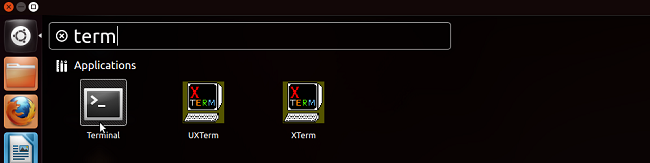
\includegraphics[width=.8\textwidth]{./images/OpenTerminal.png}

\begin{itemize}
\item \textbf{Click on the ``Terminal'' icon} as shown above
\item In the terminal, \textbf{type this line exactly as shown}:
\end{itemize}
{\footnotesize
\begin{verbatim}
 cd; wget http://tinyurl.com/stata-graphics-zip; unzip stata-graphics-zip
\end{verbatim}
\normalsize}

\begin{itemize}
\item If you see ``ERROR 404: Not Found'', then you mistyped the command -- try again, making sure to type the command exactly as shown
\end{itemize}
\end{frame}
\begin{frame}[fragile]
\frametitle{Launch Stata on Athena}
\label{sec-1-3}


\begin{itemize}
\item To start Stata \textbf{type these commands in the terminal}:
\end{itemize}
\begin{verbatim}
     add stata
     xstata
\end{verbatim}
\begin{itemize}
\item Open up today's Stata script
\begin{itemize}
\item In Stata, go to \textbf{Window => New do file => Open}
\item Locate and open the \texttt{StatGraphics.do} script in the StataStatistics folder in your home directory
\end{itemize}
\item I encourage you to add your own notes to this file!
\end{itemize}
\end{frame}

\end{document}
